% chap2.tex

\chapter{Electric Ray Robot}\label{chap:eray}

Electric Ray robot developed by Protocentral Inc, as shown in Figure~\ref{fig:electric}, is an Arduino compatible~\cite{eray} robot. It is an entry-level, low-cost complete robotic platform. It is simple enough to be used out-of-the-box for teaching and learning robotics and Arduino programming.  

\begin{figure}[h]
\centering
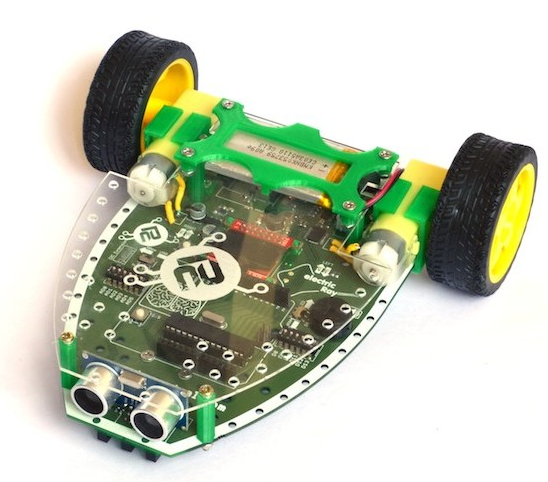
\includegraphics[width=0.5\columnwidth]{Images/electric_ray}
\caption{Electric Ray Robot}
\label{fig:electric}
\end{figure}

\section {Specification Summary}

\begin{itemize}
    \item Atmega328 microcontroller with Optiboot bootloader (Arduino-Uno compatible)
    \item Arduino shield expansion headers
    \item Ultrasonic distance sensor
    \item 3x IR sensors
    \item OLED display
    \item Piezo buzzer
    \item FTDI USB-to-serial coverter
    \item TB6612FNG Motor Driver
    \item 2x 3V geared motors
    \item 2x wheels with rubber tyres
    \item 1100 mAH, 3.7V Li-Poly battery pack
    \item Clear acrylic sheet to cover the PCB
\end{itemize}

\section{Component Details}

The electric Ray robot is a single PCB-based platform which includes all the components required for a basic robotics project including microcontroller, sensors, motors, motor drivers and power supply. 

From the top, an ultrasonic distance sensor module is placed in the front of the robot to measure the distance to the nearest obstacle in the robot's path. This produces a digital echo signal proportional to the distance to the closest object. On the bottom of the board at the same place, three IR sensors are mounted for line detection and following. 

The ATmega328 (running at 16 MHz at 5V power) microcontroller onboard contains a Arduino-Uno compatible Optiboot bootlaoder that allows you to upload code through the Arduino IDE. The onboard FTDI USB-to-serial converter IC enables the connection of the microcontroller's serial port to the PC's USB port for programming and serial data transfer. Also connected to this microcontroller are female headers with a standard Arduino Uno footprint to take any Arduino shield compatible with the Arduino Uno. 

A 2-color 128x64 pixels 0.96" Organic LED (OLED) display is present to display any messages from the code. This is connected to the ATmega328 through an SPI interface. The Adafruit SSD1306 OLED driver library can be used to control this display. An LED is also available onboard for user control and indication. 

The motor driver is based on the TB6612FNG chip which is capable of driving two DC motors at up to 1.2 A continuous current. This driver controls two 3V DC motors with integrated gearboxes for speed control. The motor driver is also capable of driving the motors at adjustable speeds and in both directions. 

Power supply is from a 3.7V, 1100 mAH Lithium-Polymer rechargeable battery pack. The 3.7V voltage is stepped up by an on-board boost DC/DC converter to the 5V required by all the components on the board. The battery can be recharged by connecting the robot to a PC through USB. Charging will continue even when the power switch is in the OFF position. Battery charging will be shut off once the battery has been completely charged. 

\begin{figure}[h]
\centering
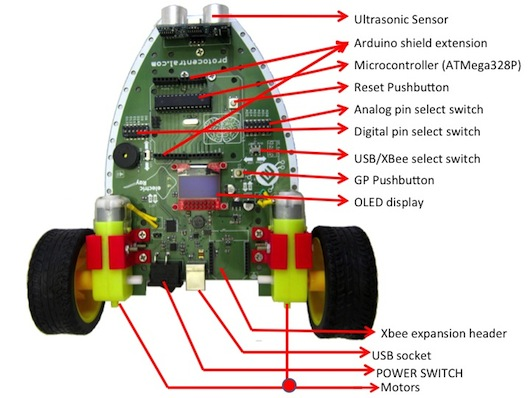
\includegraphics[width=0.75\columnwidth]{Images/electric_ray_parts}
\caption{Electric Ray Robot}
\label{fig:electric_ray_parts}
\end{figure}

\section{Programming the robot}

To program the robot, connect the robot to your computer via USB. Open the Arduino IDE, and load the sketch located in Appendix~\ref{apdx:b}.

\begin{figure}[h]
\centering
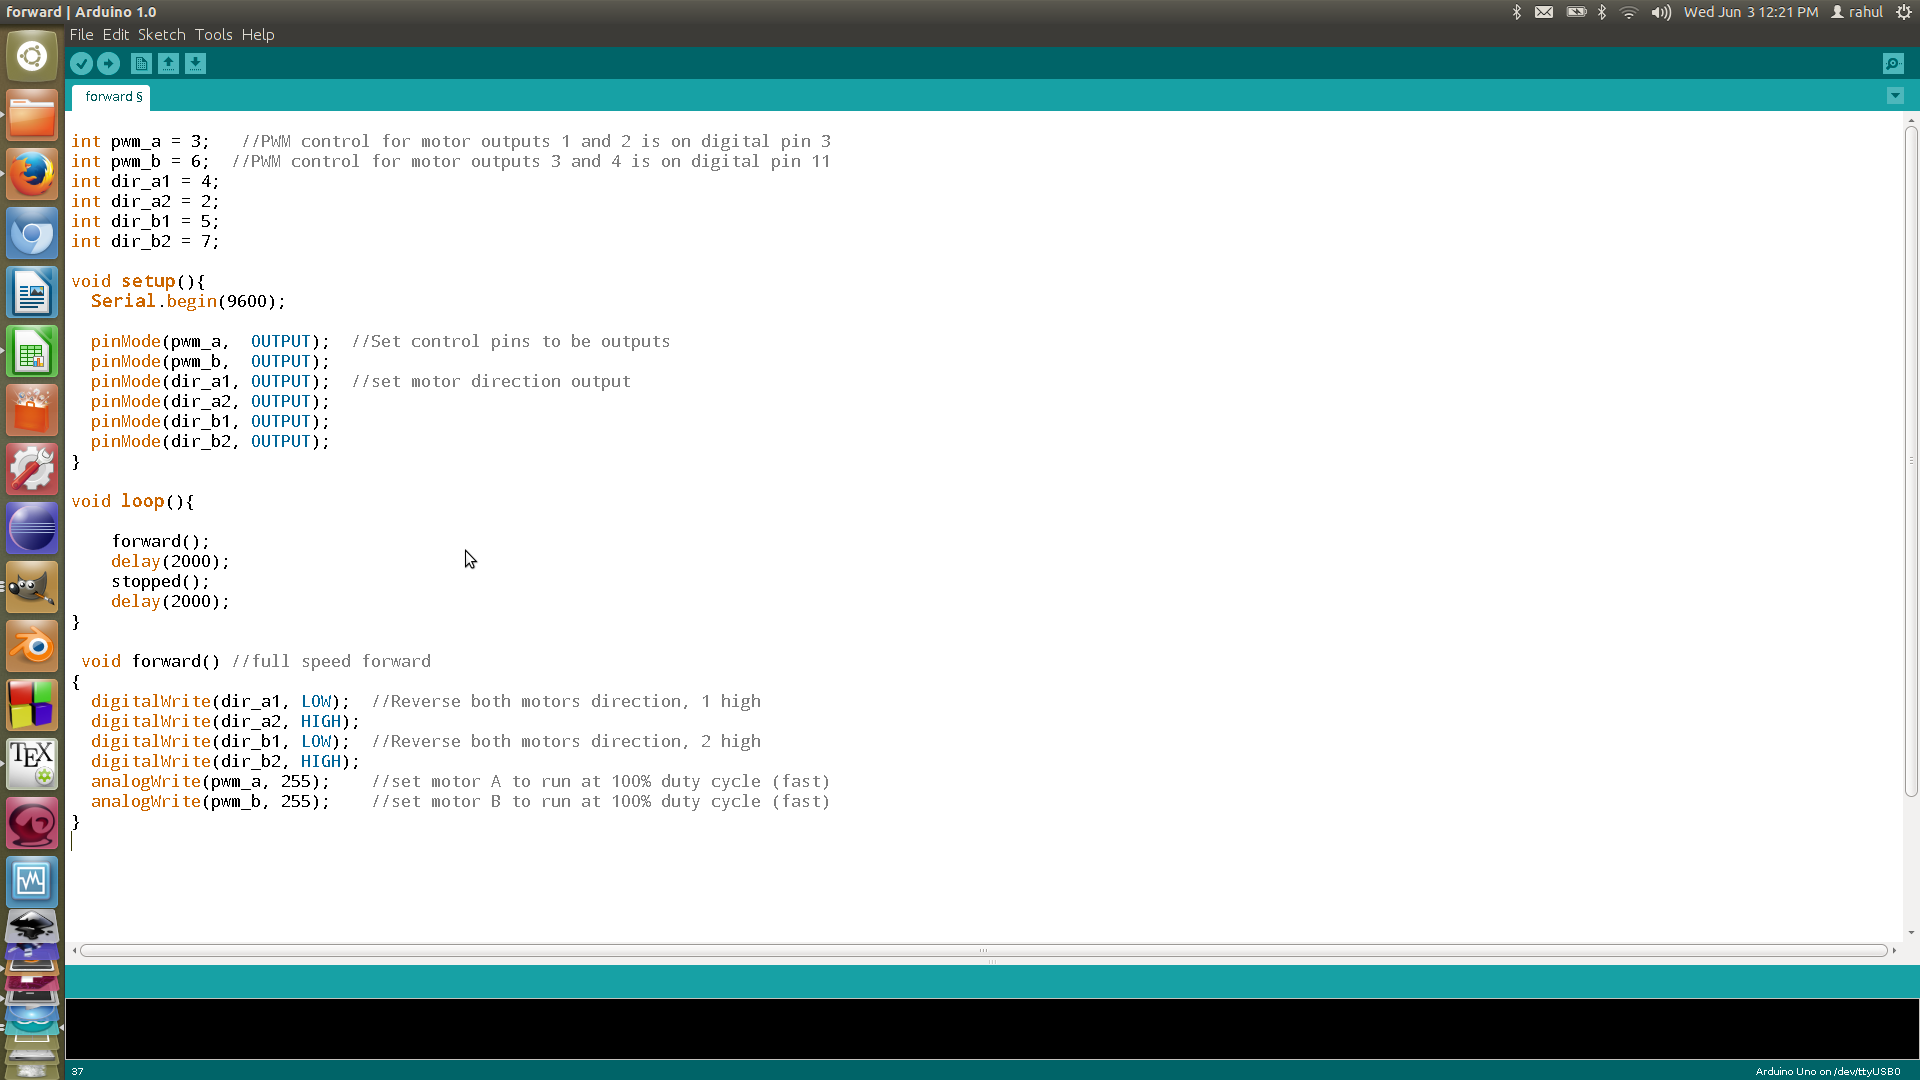
\includegraphics[width=1\columnwidth]{Images/arduino}
\caption{Arduino IDE}
\label{fig:arduino}
\end{figure}

You need to tell the IDE which Arduino board you are targeting with your software, so open the Tools - Board menu and choose Arduino Uno.

The Arduino IDE must know which of your USB ports the robot is connected to. The Tools - Serial Port menu lists the available ports. If only one item is shown, click on that one.
If two or more are shown, you can disconnect the robot and re-open the menu; the entry that disappears should be the robot. Reconnect the board and select that serial port. 

Click the "Upload" button in the top left of the IDE window. Wait a few seconds - you should see the RX and TX leds on the board flashing. If the upload is successful, the message "Done uploading." will appear in the status bar of the software. Once this appears, you can disconnect the robot from the USB cable

With batteries in the robot, turn on the power switch and put it on the ground. The robot should start moving forward.

